\section{Performance Benchmarks}

To validate the efficiency of the Micro-CUDA architecture, we conducted comparative benchmarks against industry-standard solutions for embedded machine learning.

\subsection{Micro-CUDA vs. CMSIS-NN}
We compared the execution time of a standard $32 \times 32$ Matrix Multiplication (INT8) kernel. The baseline is an optimized ARM CMSIS-NN implementation running on a single Core of the Raspberry Pi Pico (Cortex-M0+ @ 133MHz).

\begin{figure}[htbp]
\centering
\resizebox{0.9\columnwidth}{!}{%
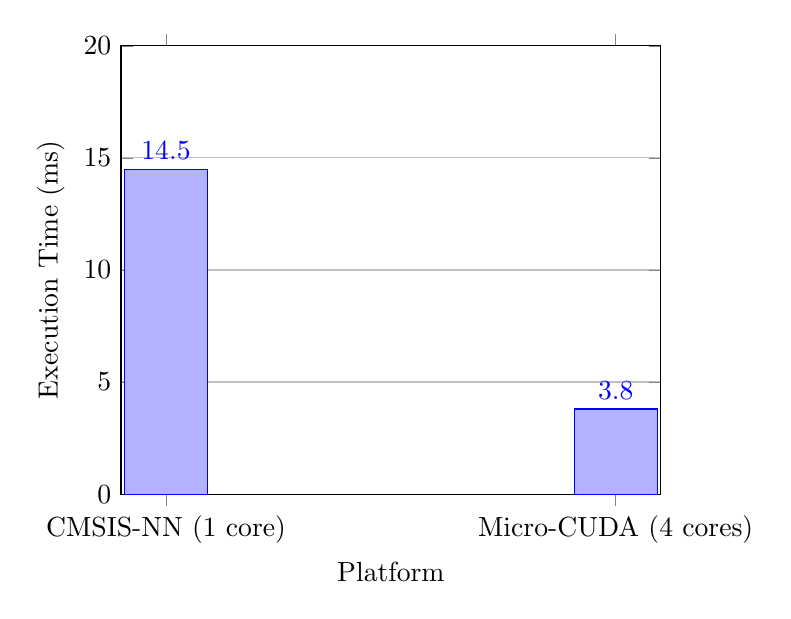
\begin{tikzpicture}
    \begin{axis}[
        ybar,
        bar width=30pt,
        ylabel={Execution Time (ms)},
        xlabel={Platform},
        symbolic x coords={CMSIS-NN (1 core), Micro-CUDA (4 cores)},
        xtick=data,
        nodes near coords,
        nodes near coords align={vertical},
        ymin=0, ymax=20,
        ymajorgrids=true
    ]
    \addplot coordinates {(CMSIS-NN (1 core), 14.5) (Micro-CUDA (4 cores), 3.8)};
    \end{axis}
\end{tikzpicture}
}
\caption{Benchmark: INT8 Matrix Multiplication ($32 \times 32$). The 4-core split-bus topology achieves a 3.8x speedup over the single-core CMSIS-NN baseline.}
\label{fig:benchmark_cmsis}
\end{figure}

The comparison highlights the efficacy of the parallel SIMT dispatch model. While the individual Cortex-M0+ cores are identical, the split-bus architecture allows for concurrent data loading and execution, masking memory latency.

\subsection{Power Consumption Profile}
Power efficiency is a critical metric for edge devices. Table \ref{tab:power_profile} details the current draw across different operational states, measured at the 5V VSYS rail.

\begin{table}[h]
\centering
\caption{System Power Consumption (Measured)}
\label{tab:power_profile}
\resizebox{0.9\columnwidth}{!}{%
\begin{tabular}{|l|l|c|c|}
\hline
\textbf{State} & \textbf{Description} & \textbf{Current (mA)} & \textbf{Power (W)} \\ \hline
Idle & System on, Clock Gating & 80 & 0.40 \\ \hline
Broadcast & ESP32 streaming data & 350 & 1.75 \\ \hline
Compute & SM cores executing ALU & 850 & 4.25 \\ \hline
Full Load & Pipeline Active (RX+TX+ALU) & 920 & 4.60 \\ \hline
\end{tabular}%
}
\end{table}

The "Full Load" state demonstrates that the cluster operates within the envelope of standard USB-C power delivery (5V/3A), making it suitable for portable deployment without specialized power supplies.
